\chapter{Derivation of the adjoint gradient and adjoint equations}\label{ch:app_adj_der}

In this appendix, we derive the adjoint equations given below in \eqref{eq:app_adjoint_momentum} -- \eqref{eq:app_adjoint_eta}:  

{\footnotesize
\begin{align}
%- \frac{\partial \bs{\xi}}{\partial t} + \big( \nabla \utilde \big)^T \bs{\xi} - \big( \utilde \cdot \nabla \big) \bs{\xi} &= - \nabla \pi / \rho - \nabla \cdot \boldsymbol{\tau}^*_{sgs} + \sum_{i=1}^{N_t} \frac{1}{2} \ctihat V_i (~3a V_i - 2 X_i ) \R_i \eperpi - \lambda \bs{\xi} \label{eq:app_adjoint_momentum}\\
- \frac{\partial \bs{\xi}}{\partial t} + \big( \nabla \utilde \big)^T \bs{\xi} - \big( \utilde \cdot \nabla \big) \bs{\xi} &= - \nabla \pi / \rho - \nabla \cdot \boldsymbol{\tau}^*_{sgs} + \sum_{i=1}^{N_t} \bs{f}^*_i - \lambda \bs{\xi} \label{eq:app_adjoint_momentum}\\
\nabla \cdot \bs{\xi} &= 0 \label{eq:app_adjoint_continuity}\\
-\tau \ddt{\sigma_i} &= -\sigma_i + \frac{1}{2} V_i^2  (a V_i - X_i) A_i \label{eq:app_adjoint_sigma}\\
- \ddt{\eta_i} &= \frac{1}{2} \ctihat V_i ~ \Bigg[ \int_{\Omega} \bigg((~3a V_i - 2 X_i ) \utilde - V_i \bs{\xi} 
\bigg) \cdot \bs{e}_{\parallel,i} \R_i \dx \nonumber \\
& \qquad  + \sint \bigg( (3a V_i - 2 X_i )~\utilde - V_i \bs{\xi} \bigg) \cdot \eperpi ~ \mathscr{Q}_i  \dx \Bigg] \label{eq:app_adjoint_eta}.
\end{align}
}

The derivation of the standard transport terms is well-known in literature (see, e.g. \citealp{choi1999instantaneous, bewley2001dns}).
Furthermore, the derivation of the adjoint Smagorinsky model and the adjoint wall-stress model is given in \cite{goit2015optimal}. Here, the derivation of the adjoint actuator disk forcing $\bs{f}_i^*$, as well as the equations for the adjoint version of the time-filtered thrust coefficient $\sigma_i$ and the adjoint yaw rate $\eta_i$ are presented. The derivation is performed using the formal Lagrangian approach (see, e.g. \citealp{borzinschulz, troltzsch}). For ease of derivation and notation, we augment the original optimization problem in Equation \eqref{eq:costfunction} with some additional trivial state constraints containing the definitions for $\R_i, \eperpi$, and $V_i$. The box constraints in \eqref{eq:boxct_constraint}--\eqref{eq:boxomega_constraint} are explicitly taken into account by the optimization algorithm as discussed in Section \ref{sec:problem_optimization}, and are omitted in the remainder of the derivation. The resulting augmented optimal control problem hence looks as follows:\footnote{Note that, throughout this text, $\delta [ a ]$ denotes the dirac delta function applied to a scalar argument $a$, whereas $\delta h$ represents a variation of a functional $h$. }

{\footnotesize
\begin{mini}[1]
	{\scriptsize \bs{\varphi}, \bs{q}}{\J(\bs{\varphi}, \bs{q}) = - \Tint \sum_{i=1}^{N_t} \frac{1}{2} C_{P,i}'~V_i^3 A_i \dt}{}{}
	\addConstraint{\small \frac{\partial \utilde}{\partial t} + \big(\utilde \cdot \nabla \big)~ \utilde }{\small = - \nabla (\ptilde + \ptilde_\infty) / \rho - \nabla \cdot \boldsymbol{\tau}_{sgs} + \sum_{i=1}^{N_t} \bs{f}_i +\bs{f}_{\rm fr}^* \ }{\small \text{in } \Omega \times (0,T] }
	\addConstraint{\small \nabla \cdot \utilde}{\small =0,}{\small \text{in } \Omega \times (0,T]}
	\addConstraint{\small \tau \ddt{\ctihat}}{\small =\cti - \ctihat}{\small i=1...N_t~\text{in } (0,T]}
	\addConstraint{\small \ddt{\theta_i}}{\small = \omega_i}{\small i=1...N_t~\text{in } (0,T]}
	\addConstraint{ \R_i(\bs{x})}{= \sint G(\bs{s} - \bs{x})~H\big[D/2 - \vert\vert \bs{s} - \bs{t}_i \vert\vert_2\big]~\diracdelta \big[ (\bs{s} - \bs{t}_i)\cdot \eperpi \big] \ds \ }{\small i=1...N_t}
	\addConstraint{\eperpi}{=\bs{e}_x \cos \theta_i  + \bs{e}_y \sin \theta_i}{i=1...N_t}
	\addConstraint{V_i}{= \vi}{i=1...N_t~\text{in } (0,T]}
\end{mini}}

Further, we define the Lagrangian of this optimization problem by adding the state constraints, with shorthand notation $\bs{B}(\bs{\varphi}, \bs{q})$, to the cost functional using the adjoint variables $\bs{q}^*$ as Lagrange multipliers as follows:

{\footnotesize 
\begin{align}
&\mathscr{L}(\bs{\varphi}, \bs{q}, \bs{q}^*) = \J(\bs{\varphi}, \bs{q}) + \innerproduct{\bf{B}(\bs{\varphi}, \bs{q})}{\bs{q}^*} \nonumber\\
&= \Tint \sum_{i=1}^{N_t} - \frac{1}{2} a \ctihat~V_i^3 A_i \dt \nonumber\\
&+ \stint \bigg\{ \frac{\partial \utilde}{\partial t} + \big(\utilde \cdot \nabla \big)~ \utilde + \nabla (\ptilde + \ptilde_\infty) / \rho + \nabla \cdot \boldsymbol{\tau}_{sgs}  - \sum_{i=1}^{N_t} \bs{f}_i - \lambda (\bs{u}_{\text{in}} - \ufilt )\bigg\} \cdot \bs{\xi} \dx \dt \nonumber\\
&+ \stint \bigg\{ \nabla \cdot \utilde \bigg\} \pi \dx \dt \nonumber\\
&+ \Tint \sumturbines \bigg\{  \tau \ddt{\ctihat} - \cti + \ctihat \bigg\} \sigma_i \dt  \nonumber\\
&+ \Tint \sumturbines \bigg\{ \ddt{\theta_i} - \omega_i \bigg\} \eta_i\dt \nonumber\\
&+ \stint \sumturbines \bigg\{ \R_i(\bs{x}) - \sint G(\bs{s} - \bs{x})~H\big[D/2 - \vert\vert \bs{s} - \bs{t}_i \vert\vert_2\big]~\diracdelta \big[ (\bs{s} - \bs{t}_i)\cdot \eperpi \big] \ds \bigg\} \rho_i \dx \dt \nonumber\\
&+ \Tint \sumturbines \bigg\{ \eperpi - \bs{e}_x \cos \theta_i  - \bs{e}_y \sin \theta_i \bigg\} \cdot \bs{\gamma}_i \dt \nonumber \label{eq:lagrangian_derivation}\\
&+ \Tint \sumturbines \bigg\{ V_i - \vi \bigg\} \chi_i \dt .
\end{align}
}

The adjoint equations in \eqref{eq:app_adjoint_momentum} -- \eqref{eq:app_adjoint_eta} can then be found by postulating vanishing gradients of the Lagrangian as  $\mathscr{L}_{\blds{q}_j}(\delta \blds{q}_j)= (\partial \mathscr{L}/\partial \blds{q}_j, \delta \blds{q}_j) = 0$ (see Equation \ref{eq:adjoint_eq_concept}) with respect to each of the state variables $\blds{q}_j$ in $\blds{q} = [\ufilt, \ptilde, \ctnhat{1}, \dots, \ctnhat{N_t}, \theta_1, \dots, \theta_{N_t}]$.  Further, given that these equations are satisfied, the gradient of the reduced cost functional can be found by simply expressing the sensitivity of the Lagrangian to the control variables as $\Lagr_{\varphi_j}(\delta \varphi_j)$ for the control parameters $\varphi_j$ in $\bs{\varphi} = [\ctn{1}, \dots, \ctn{N_t}, \omega_1, \dots, \omega_{N_t}]$ (see Equation \ref{eq:adjoint_grad_concept}).

In the following sections, firstly the adjoint gradient is derived. Thereafter, we derive the adjoint time-filtered thrust equation \eqref{eq:app_adjoint_sigma}, followed by the forcing terms for the adjoint turbine model and fringe region. Lastly, the derivation of the adjoint yaw angle equation \eqref{eq:app_adjoint_eta} is presented. 


\section{Adjoint gradient}
The cost functional gradient $\nabla \Jtilde$ can be found trivially by evaluating the derivative of the Lagrangian in \eqref{eq:lagrangian_derivation} with respect to the thrust setpoints and yaw rate controls as 
\begin{align}
	&\Lagr_{\cti}(\delta\cti) = \innerproductsmall{\partial \Lagr /\partial \cti}{\delta \cti} = \Tint -\sigma_i \ \delta \cti \dt, \label{eq:app_adjoint_grad_sigma}\\
	&\Lagr_{\omega_i}(\delta\omega_i) = \innerproductsmall{\partial \Lagr /\partial \omega_i}{\delta \omega_i} = \Tint -\eta_i \ \delta \omega_i \dt. \label{eq:app_adjoint_grad_eta}
\end{align}

Hence leading to the gradient expression given in \eqref{eq:problem_gradient}
\begin{equation}
\nabla \Jtilde \equiv 
\begin{bmatrix*}[l]
\partial \Jtilde / \partial \bs{C}_T' \\
\partial \Jtilde / \partial \bs{\omega} 
\end{bmatrix*} = 
\begin{bmatrix}
- \bs{\sigma}\\
- \bs{\eta}
\end{bmatrix}
\end{equation}



\section{Adjoint of time-filtered thrust coefficient}
We find the adjoint time filter equation by expressing the Riesz representation of $\mathscr{L}_{\widehat{\blds{C}}_T'} (\delta \widehat{\blds{C}}_T') = 0$. Using equations \eqref{eq:lagrangian_derivation}, \eqref{eq:costfunction}, \eqref{eq:define_force} and \eqref{eq:define_power}, and applying partial integration to the transient term leads to

{\footnotesize
\begin{align}
&\mathscr{L}_{\widehat{\blds{C}}_T'}(\delta {\widehat{\blds{C}}_T'}) = \mathscr{J}_{\widehat{\blds{C}}_T'}(\delta \widehat{\blds{C}}_T') - \int_0^T \int_\Omega \blds{f}_{\widehat{\blds{C}}_T'} \cdot \blds{\xi}~\dx~\dt + \int_0^T \sum_{i=1}^{N_t} \bigg( \tau \ddt{\delta \widehat{C}_{T,i}'} + \delta \widehat{C}_{T,i}' \bigg) \sigma_i \dt\\
&= \int_0^T \int_\Omega \sum_{i=1}^{N_t} \frac{1}{2} V_{i}^2 \mathscr{R}_i(\blds{x}) \bigg( -\dd{C_{P,i}'}{\widehat{C}_{T,i}'}~\ufilt + \blds{\xi} \bigg)  \cdot \blds{e}_\perp \  \delta \widehat{C}_{T,i}'~\dx~\dt \nonumber\\
& \qquad \qquad + \int_0^T \sum_{i=1}^{N_t} \bigg( \tau \ddt{\delta \widehat{C}_{T,i}'} + \delta \widehat{C}_{T,i}' \bigg) \sigma_i~\dt \\ 
&= \int_0^T \sum_{i=1}^{N_t} \bigg( -\tau \ddt{\sigma_i} + \sigma_i + \frac{1}{2} V_{i}^2 \int_\Omega \mathscr{R}_i(\blds{x}) (-a~\ufilt + \blds{\xi}) \cdot \blds{e}_\perp~\dx \bigg) \delta \widehat{C}_{T,i}'~\dt \nonumber\\
& \qquad \qquad + \sum_{i=1}^{N_t} \tau \bigg[\delta \widehat{C}_{T,i}'\ \sigma_i \bigg]_0^T.    
\end{align}
}

By equalizing the above expression to zero, and imposing the terminal condition $\sigma_i(T)=0$, we recover the adjoint equation for $\sigma_i$: 
\begin{equation}
	-\tau \ddt{\sigma_i} = -\sigma_i + \frac{1}{2} V_i^2  (a V_i - X_i) A_i
\end{equation}


\section{Adjoint turbine forcing term}
The adjoint turbine forcing term, which is the driving source term in the adjoint equations, is found as follows:
\begin{align}
&\big( -\blds{f}^*, \delta \ufilt \big) = \mathscr{J}_{\ufilt} (\delta \ufilt) + \int_{0}^{T} \int_\Omega -\blds{f}_{\ufilt} (\delta \ufilt) \cdot \blds{\xi}~\dx~\dt\\
&= \int_{0}^{T} \int_{\Omega} \sum_{i=1}^{N_t} -\frac{3}{2} C_{P,i}' V_{i}^2 \mathscr{R}_i (\blds{x}) \blds{e}_\perp \cdot \delta \ufilt~\dx~\dt \nonumber \\
& \qquad + \int_{0}^{T} \int_{\Omega} \sum_{i=1}^{N_t} \widehat{C}_{T,i}' V_{i} \bigg( \frac{1}{A_i} \int_{\Omega} \mathscr{R}_i(\blds{x}) \blds{\xi} \cdot \blds{e}_\perp \dx  \bigg) \mathscr{R}_i (\blds{x}) \blds{e}_\perp \cdot \delta \ufilt ~\dx~\dt\\
&= \int_{0}^{T} \int_{\Omega} \sum_{i=1}^{N_t} -\frac{1}{2} \widehat{C}_{T,i}' V_{i} \bigg(3~\frac{C_{P,i}'}{\widehat{C}_{T,i}'}~V_{i} - 2~X_{i} \bigg)~\mathscr{R}_i (\blds{x}) \blds{e}_\perp \cdot \delta \ufilt ~\dx~\dt\\
&= \int_{0}^{T} \int_{\Omega} \sum_{i=1}^{N_t} -\frac{1}{2} \widehat{C}_{T,i}' V_{i} \bigg(3~a~V_{i} - 2~X_{i} \bigg)~\mathscr{R}_i (\blds{x}) \blds{e}_\perp \cdot \delta \ufilt ~\dx~\dt,
\end{align}
hence leading to the definition of the adjoint forcing term for turbine $i$ as 
\begin{equation}
	\bs{f}_i^* = \frac{1}{2} \widehat{C}_{T,i}' V_{i} \bigg(3~a~V_{i} - 2~X_{i} \bigg)~\mathscr{R}_i (\blds{x}) \blds{e}_\perp.
\end{equation}

\section{Adjoint fringe region forcing term}
It was shown in Chapter \ref{ch:methodology} that the fringe forcing term, defined as $\bs{f}_{\text{fr}} = \lambda (\ufilt_{\text{in}} - \ufilt)$ forces the flow field $\ufilt$ to the desired inlet boundary condition $\ufilt_{\text{in}}$. The adjoint fringe forcing $\bs{f}_{\text{fr}}^*$ can be found as:

\begin{align}
	\innerproductsmall{\bs{f}_{\text{fr}}^*}{\delta \ufilt} &= \stint \bigg\{ -\lambda \ \delta \ufilt\bigg\}\cdot \bs{\xi}~ \dx \dt
\end{align}

hence $\bs{f}_{\text{fr}}^* = -\lambda \bs{\xi}$. This expression also follows from intuition, as the fringe region dampens out the turbine wakes and replaces them with independently generated inlet conditions in the forward simulation, so will the adjoint solution be damped to zero by the adjoint fringe force, indicating that the influence of the wind-farm behavior does not extend over the upstream domain boundary. 

\section{Adjoint of yaw angle}
The current section discusses the derivation of the adjoint yaw angle Equation \eqref{eq:app_adjoint_eta}. This derivation is somewhat more complex than the ones presented above. Therefore, to keep notations concise and the derivation clear, we will proceed by first deriving some auxiliary adjoint equations for the rotor footprint $\R_i$ and the disk velocity $V_i$. These will yield straightforward algebraic expressions for the adjoint variables $\rho_i$ and $\chi_i$ respectively, which will be substituted within the derivation of the equation for the adjoint rotor-perpendicular vector $\bs{\gamma}_i$. Thereafter, the adjoint yaw angle equation for the adjoint variable $\eta_i$ will follow in a straightforward manner.



\subsection{Adjoint disk velocity equation}
The adjoint disk velocity equation for the adjoint variable $\chi_i$ is found by equating the functional derivative of the Lagrangian $\Lagr$ to the disk velocity $V_i$ to zero for $i = 1 \dots N_t$: 
\begin{align}
\Lagr_{V_i}(\delta V_i) = \innerproductsmall{\partial \Lagr / \partial V_i}{\delta V_i} &= \Tint -\frac{1}{2} a \ctihat 3 V_i^2 A_i \delta V_i \dt  \nonumber \\
& \ \ + \Tint \frac{1}{2} \ctihat 2 V_i X_i  A_i \delta V_i \dt \nonumber \\
& \ \ + \Tint \chi_i \delta V_i \dt = 0, 
\end{align}
which yields the following expression for the adjoint variable $\chi_i$:
\begin{equation}\label{eq:chi_i}
\chi_i = \frac{1}{2} \ctihat V_i (~3a V_i - 2 X_i )~A_i \qquad\qquad \text{for } i=1\dots N_t 
\end{equation}

\subsection{Adjoint rotor footprint equation}
Similary, the adjoint rotor footprint equation for the adjoint variable $\rho_i$ is found by expressing the derivative of the Lagrangian $\Lagr$ to the footprint $\R_i$: 
\begin{align}
\Lagr_{\R_i}(\delta \R_i) = \innerproductsmall{\partial \Lagr / \partial \R_i}{\delta \R_i} &= 
\stint \frac{1}{2} \ctihat V_i^2 \eperpi \cdot \bs{\xi} \delta \R_i ~\dx \dt \nonumber \\
& \ \ + \stint \rho_i \delta \R_i ~\dx \dt \nonumber \\
& \ \ + \stint -\frac{\chi_i}{A_i} \utilde \cdot \eperpi \delta \R_i ~\dx \dt = 0,
\end{align}    
leading to a straightforward expression of the adjoint variable $\rho_i$:
\begin{align}
\rho_i &= \bigg( \frac{\chi_i}{A_i}~\utilde - \frac{1}{2} \ctihat V_i^2 \bs{\xi} \bigg) \cdot \eperpi \label{eq:rho_i_1}  \\
 &= \frac{1}{2} \ctihat V_i \bigg(3aV_i \ufilt  -2 X_i \ufilt - V_i\bs{\xi} \bigg) \cdot \eperpi \qquad\qquad \text{for } i=1\dots N_t. \label{eq:rho_i}
\end{align}

\subsection{Adjoint perpendicular vector equation}

{\small
\begin{align}
&\Lagr_{\R_i}(\delta \R_i) =\innerproductsmall {\partial \Lagr / \partial \eperpi}{\delta \eperpi} = \nonumber \\
& \stint \frac{1}{2} \ctihat V_i^2 \R_i \bs{\xi} \cdot \delta \eperpi \dx \dt \nonumber \\
& + \stint - \rho_i \times \nonumber \\
& \qquad \bigg\{ \sint G(\bs{s} - \bs{x})  H\big[D/2 - \vert\vert \bs{s} - \bs{t}_i \vert\vert_2 \big]~\diracdelta'\big[(\bs{s} - \bs{t}_i) \cdot \eperpi \big]~(\bs{s} - \bs{t}_i) \cdot \delta \eperpi \ds \bigg\} \dx \dt \nonumber\\
& + \Tint \bs{\gamma}_i \cdot \delta \eperpi \dt \nonumber \\ 
& + \stint -\frac{\chi_i}{A_i} \R_i \utilde \cdot \delta \eperpi \dx \dt \label{eq:app_adj_perp1}.
\end{align}}

The second term in the expression above requires some further attention. The derivative operator on the dirac delta function can be transferred to the other terms using partial integration by invoking a coordinate transformation from  the LES reference frame $(\bs{e}_x, \bs{e}_y, \bs{e}_z)$ to the rotor reference frame\footnote{From this point onward in the derivation, it is assumed that the rotor does not tilt. The derivation can however be generalized for rotor tilt control at the cost of somewhat more complex equations.} $(\eperpi, \etransi, \bs{e}_z)$, defining a new integration variable $\bs{\zeta} = R\bs{s}$ with $R$ a rotation matrix from the LES to the rotor reference. In doing so, the term between brackets in Equation \eqref{eq:app_adj_perp1} can be rewritten as 

\begin{align}
	&\sint G(\bs{s} - \bs{x})  H\big[D/2 - \vert\vert \bs{s} - \bs{t}_i \vert\vert_2 \big]~\frac{\text{d}\diracdelta\big[(\bs{s} - \bs{t}_i) \cdot \eperpi \big]}{\text{d} (\bs{s} - \bs{t}_i) \cdot \eperpi}~(\bs{s} - \bs{t}_i)  \ds \label{eq:app_adj_der_partial}\\
	= &\sint G(\bs{\zeta} - R\bs{x})  H\big[D/2 - \vert\vert \bs{\zeta} - R\bs{t}_i \vert\vert_2 \big]~\frac{\text{d}\diracdelta\big[(\zeta_1 - R\bs{t}_i \cdot \hat{\bs{\zeta}}_1 \big]}{\text{d}\zeta_1}~(\bs{\zeta} - R\bs{t}_i) \dzeta \nonumber\\
	= & - \sint \frac{\text{d}}{\text{d}\zeta_1} \bigg\{ G(\bs{\zeta} - R\bs{x})  H\big[D/2 - \vert\vert \bs{\zeta} - R\bs{t}_i \vert\vert_2 \big] (\bs{\zeta} - R\bs{t}_i)  \bigg\} \diracdelta\big[(\zeta_1 - (R\bs{t}_i)_1 \big]~ \dzeta,
\end{align}
where the boundary terms drop out by the definition of the dirac delta function. Furthermore, using the chain rule and properties of the dirac delta function\footnote{The term associated with the derivative of the Heaviside function H drops out since it can be rewritten in the form $\int_{-\infty}^{\infty} f(x) x \diracdelta(x)\ \dx$, which vanishes for every bounded function $f(x)$ with compact support.} the integrand in the expression above can be written as
{\small
\begin{align*}
	 G(\bs{\zeta} - R\bs{x})  H\big[D/2 - \vert\vert \bs{\zeta} - R\bs{t}_i \vert\vert_2 \big] \diracdelta\big[(\zeta_1 - (R\bs{t}_i)_1 \big] \bigg\{ \hat{\bs{\zeta}}_1 - \frac{12 \zeta_1 - (R\bs{x})_1}{\Delta^2} (\bs{\zeta} - R \bs{t}_i) \bigg\}.
\end{align*}}

\noindent Transforming back to the original LES reference frame this yields
{\small
\begin{align*}
G(\bs{s} - \bs{x})  H\big[D/2 - \vert\vert \bs{s} - \bs{t}_i \vert\vert_2 \big] \diracdelta\big[(\bs{s} - \bs{t})\cdot \eperpi \big] \bigg\{ \eperpi - \frac{12 (\bs{s} - \bs{x})\cdot \eperpi}{\Delta^2} (\bs{s} - \bs{t}_i) \bigg\}.
\end{align*}}

Substituting the integrand back into Equation \eqref{eq:app_adj_der_partial}, and defining an auxiliary variable $\bs{Q}_i = \sint \frac{12 (\bs{s} - \bs{x})\cdot \eperpi}{\Delta^2} (\bs{s} - \bs{t}_i) G(\bs{s} - \bs{x})  H\big[D/2 - \vert\vert \bs{s} - \bs{t}_i \vert\vert_2 \big] \diracdelta\big[(\bs{s} - \bs{t})\cdot \eperpi \big] \ds$ for ease of notation, we find
{\small 
\begin{align}
\sint G(\bs{s} - \bs{x})  H\big[D/2 - \vert\vert \bs{s} - \bs{t}_i \vert\vert_2 \big]~\diracdelta'\big[(\bs{s} - \bs{t}_i) \cdot \eperpi \big]~(\bs{s} - \bs{t}_i)  \ds 
=  - \R_i \eperpi + \bs{Q}_i. \label{eq:subs_this}
\end{align}}

\noindent Substituting Equation \eqref{eq:subs_this} into Equation \eqref{eq:app_adj_perp1} for the functional derivative, along with the expressions for $\rho_i$ \eqref{eq:rho_i} and $\chi_i$ \eqref{eq:chi_i} yields:
\begin{align}
&\Lagr_{\R_i}(\delta \R_i) = \Tint \bs{\gamma}_i \cdot \delta \eperpi \dt \nonumber\\
& - \stint \frac{1}{2} \ctihat V_i \bigg\{ 3a V_i \ufilt  - 2 X_i \ufilt - V_i\bs{\xi}   \bigg\} \R_i \cdot \delta \eperpi \dx \dt \nonumber \\
& + \stint \frac{1}{2} \ctihat V_i \bigg\{ \bigg(3aV_i \ufilt  -2 X_i \ufilt - V_i\bs{\xi} \bigg) \cdot \eperpi \bigg\} \R_i \eperpi \cdot \delta \eperpi \ds \nonumber \\
& - \stint \frac{1}{2} \ctihat V_i \bigg\{ \bigg(3aV_i \ufilt  -2 X_i \ufilt - V_i\bs{\xi} \bigg) \cdot \eperpi \bigg\} \bs{Q}_i \cdot \delta \eperpi \ds 
\end{align}
Since there is no rotor tilt, and the vectorial integrands of the second and third term are hence two-dimensional, their difference is simply the rotor-transversal component of the integrand, 
\begin{align}
&\Lagr_{\R_i}(\delta \R_i) = \Tint \bs{\gamma}_i \cdot \delta \eperpi \dt \nonumber\\
& - \stint \frac{1}{2} \ctihat V_i \bigg\{ \bigg(3a V_i \ufilt  - 2 X_i \ufilt - V_i\bs{\xi} \bigg) \cdot \etransi   \bigg\} \R_i \etransi \cdot \delta \eperpi \dx \dt \nonumber \\
& - \stint \frac{1}{2} \ctihat V_i \bigg\{ \bigg(3aV_i \ufilt  -2 X_i \ufilt - V_i\bs{\xi} \bigg) \cdot \eperpi \bigg\} \bs{Q}_i \cdot \delta \eperpi \ds 
\end{align}
Equating to zero finally yields the expression for the adjoint rotor-perpendicular vector $\bs{\gamma}_i$:
\begin{align}
\bs{\gamma}_i = \frac{1}{2} \ctihat V_i \sint \bigg[ & \bigg\{ \bigg(3a V_i \ufilt  - 2 X_i \ufilt - V_i\bs{\xi} \bigg) \cdot \etransi   \bigg\} \R_i \etransi   \nonumber\\
  + & \bigg\{ \bigg(3aV_i \ufilt  -2 X_i \ufilt - V_i\bs{\xi} \bigg) \cdot \eperpi \bigg\} \bs{Q}_i \bigg] \ds. \label{eq:app_adj_gamma_final}  
\end{align}

\subsection{Adjoint yaw angle equation}
The current section derives the adjoint equation for the adjoint yaw angle $\eta_i$, required for the evaluation of the cost functional yaw sensitivity in Equation \eqref{eq:app_adjoint_grad_eta}. Similar to previous sections, the derivation starts by expressing the functional derivative of the Lagrangian to the yaw angle $\theta_i$: 
\begin{align}
\Lagr_{\theta_i}(\delta \theta_i) &= 
\Tint \bs{\gamma}_i \cdot \bigg\{ \bs{e}_x \sin \theta_i - \bs{e}_y \cos \theta_i  \bigg\} \delta \theta_i \dt + \Tint \ddt{\delta \theta_i} \eta_i \dt \\ 
&= \Tint \bigg\{ -\ddt{\eta_i} + \etransi \cdot \bs{\gamma}_i   \bigg\} \dt,
\end{align}
Where partial integration on the time derivative is perform, and a terminal condition $\eta_i(T) = 0$ is applied, leading to vanishing boundary terms. This yields an ODE for $\eta_i$:
\begin{equation}\label{eq:app_adj_eta_basic}
- \ddt{\eta_i} = \bs{e}_{\parallel,i} \cdot \bs{\gamma}_i 
\qquad\qquad \text{for } i=1\dots N_t.
\end{equation}
Substituting the expression for $\bs{\gamma}_i$ from Equation \eqref{eq:app_adj_gamma_final}, this expression can be rewritten as 
\begin{align}
- \ddt{\eta_i} =  \frac{1}{2} \ctihat V_i \sint \bigg[ & \bigg\{ \bigg(3a V_i \ufilt  - 2 X_i \ufilt - V_i\bs{\xi} \bigg) \cdot \etransi   \bigg\} \R_i  \nonumber\\
+ & \bigg\{ \bigg(3aV_i \ufilt  -2 X_i \ufilt - V_i\bs{\xi} \bigg) \cdot \eperpi \bigg\} \mathscr{Q}_i \bigg] \ds. \label{eq:app_adj_eta_final} 
\end{align}
which is the adjoint equation for $\eta_i$ featured in Equation \eqref{eq:app_adjoint_eta}. In this equation, the shorthand notation for the filter kernel $\mathscr{Q}_i$ is introduced as:
{\small
\begin{align}
	& \mathscr{Q}_i = \bs{Q}_i \cdot \etransi \nonumber \\
	&= \sint \frac{12 (\bs{s} - \bs{x})\cdot \eperpi}{\Delta^2} G(\bs{s} - \bs{x})  H\big[D/2 - \vert\vert \bs{s} - \bs{t}_i \vert\vert_2 \big] \diracdelta\big[(\bs{s} - \bs{t})\cdot \eperpi \big]  (\bs{s} - \bs{t}_i) \cdot \etransi \ds.
\end{align}}

Figure \ref{fig:filters} illustrates both the original filter kernel $\R$ and the new filter kernel $\mathscr{Q}_i$. It can be seen from the figure that $\mathscr{Q}_i$ quantifies the rate of change in the rotor geometrical footprint $\R_i$ upon perturbing the yaw angle $\theta$. Therefore, $\mathscr{Q}_i$ can be regarded as a yaw-sensitivity footprint.
Further, given Equation \eqref{eq:app_adjoint_grad_eta}, it can be seen that the right-hand-side of Equation \eqref{eq:app_adj_eta_final} acts as a driving term for the yaw rate sensitivity. The first term in the right-hand-side is associated with the flow currently parallel to the rotor, which is hence not captured given the current orientation, imposing an incentive for reorientation of the rotor. The second on the other hand is associated with the flow perpendicular to the rotor just outside the rotor plane. This term causes an incentive for yawing since a change in rotor locus (i.e. where the flow field is sampled by the ADM) would allow power to be extracted from these terms. 

\begin{figure}
	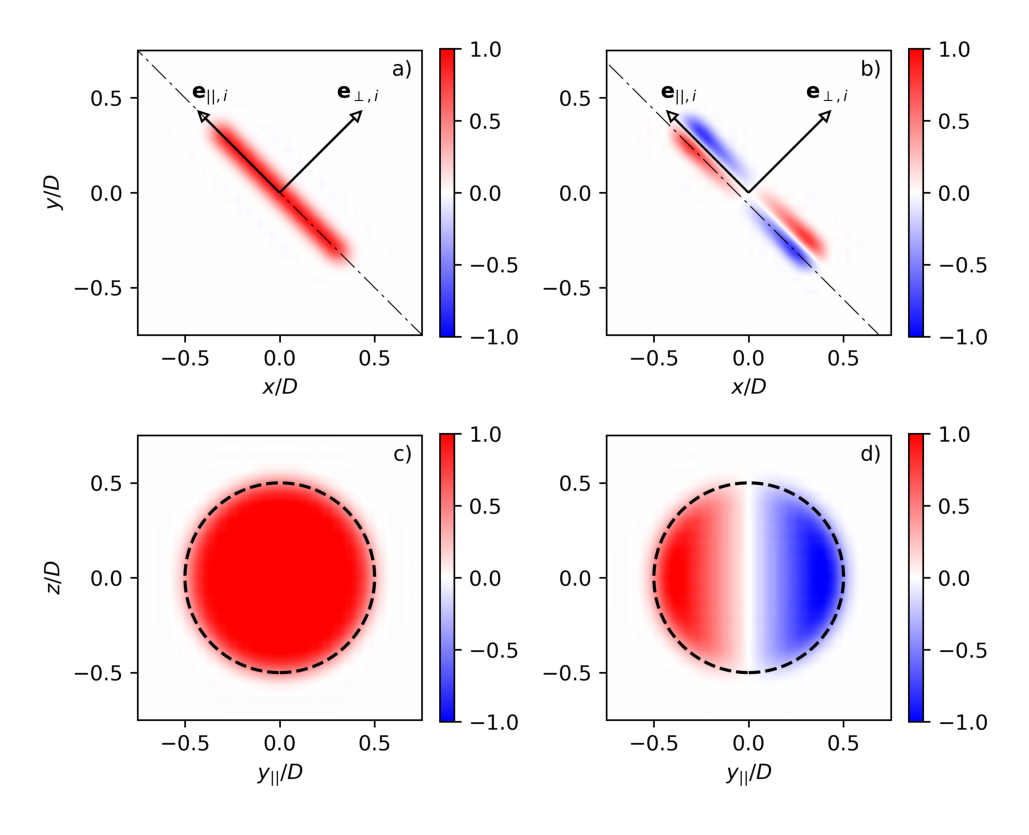
\includegraphics[width=\textwidth]{chapters/appendix_adjoint_derivation/R_Qpng.eps}
	\caption[Illustration of geometrical filter kernels in Equation \eqref{eq:app_adj_eta_final}.]{Geometrical filter kernels in Equation \eqref{eq:app_adj_eta_final}. \emph{a,c)} Original stationary rotor footprint $\R$. \emph{b,d)} New yaw-sensitivity footprint $\mathscr{Q}$. \emph{a,b)} Planview at hub height. \emph{c,d)} Cross section through plane indicated by dot dashed line in \emph{a},\emph{b}. \label{fig:filters}}
\end{figure}

\cleardoublepage